
% Chapter 1

\chapter{An Introduction to Mechanism Design Theory} % Main chapter title

\label{Chapter1} % For referencing the chapter elsewhere, use \ref{Chapter1} 

%----------------------------------------------------------------------------------------

% Define some commands to keep the formatting separated from the content 
\newcommand{\keyword}[1]{\textbf{#1}}
\newcommand{\tabhead}[1]{\textbf{#1}}
\newcommand{\code}[1]{\texttt{#1}}
\newcommand{\file}[1]{\texttt{\bfseries#1}}
\newcommand{\option}[1]{\texttt{\itshape#1}}

\newtheorem{definition}{Definition}
\newtheorem*{definition*}{Definition}
\newtheorem{thm}{Theorem}
\newtheorem*{thm*}{Theorem}
\newtheorem{example}{Example}
\newtheorem*{example*}{Example}
\newtheorem{lemma}{Lemma}
\newtheorem*{lemma*}{Lemma}
\newtheorem{prop}{Proposition}
\newtheorem*{prop*}{Proposition}
\newtheorem{assumption}{Assumption}
\newtheorem*{assumption*}{Assumption}
\newtheorem{corollary}{Corollary}
\newtheorem*{corollary*}{Corollary}
\newtheorem{conjecture}{conjecture}
\newtheorem*{conjecture*}{conjecture}
\newtheorem*{remark}{Remark}



%----------------------------------------------------------------------------------------


 
%------------------------------------------------------------------------------------------




%----------------------------------------------------------------------------------------

\section{Introduction}

The starting point of analysis in traditional economics is often the
present state of economic institutions and mechanisms, for example,
market theory, auctions and resource allocation. In mechanism design
theory, an alternative framework and perspective is used. We view the
present state of affairs just as a possibility and has an intention to
design a better mechanism with respect to a social goal or
criterion. Mechanism design is kind of engineering side of
economics. To do that, a framework must be provided. Now the framework
has become a theory with a large body of literatures. That theory is
mechanism design theory. The mechanism design theory was established
by leonid Hurwicz, later expanded by Roger B.Myerson, Eric S. Maskin,
Guoqiang Tian and many other  scholars of the field.

 The most important
component of Mechanism design theory is implementation
theory. \parencite{Liang2010} has done a survey of this field
.  The present paper is not another attempt to summarize the
implementation theory of mechanism design, but uses it as  a central tool for formalizing ideas
in this paper. This paper aims  to analyze some
economic mechanisms for situations where information  is not
fully known to the social planner. In the process, the author creates some new
concepts which the author thought is necessary. However, a little
background of the mechanism design theory is needed. This is what the next
section is about.

\section{A survey of the background}

A formal study of the informational requirements and informational optimality of resource
allocation processes was initiated by Hurwicz (1960).  In line with the prevailing tradition, interest in this area was focused
on the design of Pareto-satisfactory (non-wasteful) and privacy-preserving mechanisms, i.e.,
mechanisms that result in Pareto efficient allocations and use informationally decentralized
decision making processes.  Allocative efficiency and informational efficiency are two highly
desired properties for an economic system to have.  The importance of Pareto optimality is
attributed to what may be regarded as a minimal welfare property. Pareto optimality requires
resources be allocated efficiently. If an allocation is not efficient, there is a waste in allocating
resources and thus at least one agent is better off without making others worse off under given
resources. Informational efficiency requires an economic system have the minimal informational
cost of operation. The informational requirements depend upon two basic components: the class
and types of economic environments over which a mechanism is supposed to operate and the
particular outcomes that a mechanism is required to realize.

For informational decentralized systems, \parencite{Hurwicz1972}
proved a very important theorem: For the neoclassical pri-
vate goods economies, there is no mechanism < M, h > that implements Pareto efficient
and individually rational allocations in dominant strategy. Consequently, any revelation
mechanism < M, h > that yields Pareto efficient and individually rational allocations is
not strongly individually incentive compatible. (Truth-telling about their preferences is not
Nash Equilibrium).

A mechanism can be viewed as an abstract planning procedure; it consists of a message
space in which communication takes place, rules by which the agents form messages, and an
outcome function which translates messages into outcomes (allocations of resources). Mecha-
nisms are imagined to operate iteratively. Attention, however, may be focused on mechanisms
that have stationary or equilibrium messages for each possible economic environment. A mecha-
nism realizes a prespecified welfare criterion (also called performance, social choice rule, or social
choice correspondence) if the outcomes given by the outcome function agree with the welfare
criterion of the stationary messages. 

\section{General model framework}
 In this section, we give the framework of analysis which will
 reappear many times later in the paper with slightly different
 forms. Our framework is comprised of 5 parts: 
 economic environments, social goals or criteria,  mechanism, 
expected outcomes(often equilbirums of all kinds), and the concept of
implementation of social goals.
The following subsections will give a detailed discussion and relative
notations of these components.
\subsection{Economic environments}
Economic environments consists of economic entities and their features
as well as the state of some relevant things in the world. The
entities are of two kinds. One is the principal (or called the social
planner),  and the other is  the agents (or called economic
participants).  Usually, we have the following notations.

$N=\{1,...,n\}$: denote the set of the agents.

$e_i\in E_i$: denote the economic feature of agent $i\in N$. It may be preferences, economic status or some other relevant feature.

$E=E_1\times \dots \times E_2$: denote the set of profiles of economic features.

 The social planner does not know much information of
the participants' profile $e$. These information are decentralized
among the agents. 
If the agents all know the whole profile $e$, then it is the perfect information case; if every agent $i$ knows his own $e_i$ and knows the distribution of $e$, then this is the imperfect information case which can be dealt with using Bayesian method; else if every agent $i$ only knows his own $e_i$, then it is only good to be dealt with using strategyproof mechanisms. The details will be in later chapters.

\subsection{Social criteria}

Given an economic environment $e$, every agents participate in economic activities, make economic decisions, pay the cost and get the profits. The social planner hope that the results satisfy some criteria.
Let us give some notations and talk about it.

$A$: denote the set of social allocations, or economic results.

$F : E \mapsto A$: denote a social criterion, or social goal, which is a correpondence from the set of environments to the set of results. Given any environment $e$, there will be a subset of $A$ that satisfy the social criterion, $F$ just denotes this function.

If randomized results on $A$ are acceptable as social results, then we can use 
$\Delta A$ instead of just $A$. 

\subsection{Mechanism for information collection}

 The social planner lacks information, so he or she need to design incentive
compatible rules of the game to induce everyone reveal their true private information. 

If the social planner knows completely the environment, then he or she
can simply choose a result that is in the set $F(A)$. However, he or
she usually does not know much about these things. That is where
mechanism for information collection functions.  A mechanism, or  a
game form, usually contains the following components.

$M_i$: denote the message space of agent $i \in N$. An agent can only emit 
message $m_i \in M_i$.

$M=M_1\times\dots\times M_n$: denote the space of message profiles. Every message profile $m=(m_1,\dots,m_n)\in M$.

$h:M\rightarrow A$: denote the assignment function for the mechanism, which assigns a result for a given message profile $m$.

$ \Gamma = \langle M,h\rangle$: denote the information collection mechanism, which is just the combination of the space of message profiles and the assignment function that lies on top of it.

Thus, a mechanism prescribes rule of the game. Every agent $i$ chooses a message
$m_i \in M_i$ to send, and then the social planner collects all the messages in the message profile $m$, and finally decides on the allocation result $h(m)$ as the social choice. The $\Gamma$ must be declared openly to let every agent know, then it is up to every agent $i$ to choose from his or her $M_i$ the $m_i$ to report.

A very important class of mechanisms is the direct revelation
mechanism(or simply called direct mechanism) in which $M_i$ is just the possible world state information 
that agent $i$ has.  later we will introduce a very important theorem
about this mechanism.
\subsection{Expected outcomes}

When a mechanism $\Gamma=\langle M, h\rangle$ is given, we have a game
with rules for the agents to report $m \in M$. The strategy of an
agent $i$ is usually denoted $\sigma^i(e_i,\Gamma)$ or $\rho^i(e_i,\Gamma)$. Taking this
form is for the reason that different environments $e_i$ may induce
$i$ to choose different message for a given mechanism $\Gamma$. For a given $\Gamma$, the $\Gamma$ in the above notation can usually
be omitted as the default $\Gamma$ is clear.
When the agents send messages to the social planner, they have strategical interaction in choosing which message to send. Now we need to know what will result from the strategical interaction, these are the expected outcomes. Usually the solution concept of equilibriums in games are ideal for this role.

Here, one point concerning the $e$ should be stressed.  There is requirement on the preference
information which is contained in $e_i$ for every $i \in N$.
When people game with each other, the hypothesis for human behavior is
very important. A fundamental hypothesis is that human being are
self-interested, that is, they will try to maximize some kind of
self-utility. With this hypothesis, it is usually implied that human
being will not deliberately contribute to the society without
considering the returns to himself or herself. Or put it another way,
a human being will only concentrate on maximizing self-interest, only
a good mechanism can make this self-interesting behavior also
beneficial to the society. Let $\succeq_{e_i}$ denote the preference
in $e_i$ for agent $i$. It must be an order relation on the results
set $A$. Put it another way, it must satisfy the following 3
conditions.

\begin{itemize}
\item Reflexivity. For any outcome $a \in A$, $a\succeq a$.
\item Completeness. For any two outcomes $a$ and $b$ from $A$, either $a\succeq
  b$ or $b\succeq a$. That is , any two outcomes are comparable.
\item Transitivity. For any three outcomes $a$, $b$ and $c$, if both
  $a \succeq b$ and $b \succeq c$ hold, then $a \succeq c$ hold. This
  eliminates unwanted circles.
\end{itemize}

Two other relations $\succ$ and $\sim$ can be generated from a given
$\succeq$.
For any $a$ and $b$ from the results set $A$, $a \succ b$ if and only
if $a \succeq b$ and $b \not \succeq a$; $a \sim b$ if and only if  $a
\succeq b$ and $b \succeq a$. 

The three relations $\succeq, \succ,\sim$ are also frequently denoted
with a single letter $R, P, I$ respectively. Later, we will use these
single letter forms for consistency with matching literature in that
chapter.


With this kind of preference, every agent $i$ can rank the results in
$A$ in such a way that equilibriums are definable.

With this hypothesis, the equilibrium concepts of game theory best suit our needs for the expected outcomes. The equilibriums are the expected outcomes. For different situations, different equilibrium concepts should be taken as the expected outcomes. Dominant strategy equilibrium, Nash equilibrium, Subgame perfect Nash equilibrium, Bayesian Nash equilibrium, Perfect Bayesian equilibrium and so on all have their chances of being the expected outcomes depending on the problem situation. Notations are as follows.

$b(e,\Gamma)$: denote the equilibrium message choices $M* \subset M$ under the economic environment $e$ and mechanism $\Gamma$.

$h(b(e,\Gamma))$: denote the expected outcomes of the assignment.

For a given $\Gamma$, the $\Gamma$ in the above notation can usually
be omitted as the default $\Gamma$ is clear.






  

\subsection{Implementation of social criteria}

Finally, comes the concept of implementation. An important goal of
mechanism design is to make individual incentives and social criteria
compatible.  Roughly speaking, if a social criteria is satisfiable under certain
equilibrium solution of a mechanism, then we say that that social
criteria is implementable with that mechanism.
The idea can be illustrated by the following graph.

\begin{center}
\begin{tikzpicture}
\draw [->] [thick] (1,0) --  (7,0);
\node [below] at (4,0) {$F(e)$};
\draw [->] [thick] (1,0)--(4,2);
\node [left] at (2.5,1) {$b(e, \Gamma)$};
\draw [->][thick] (4,2)--(7,0);
\node [right] at (5.5,1) {$h(b(e,\Gamma))$};

\node [above] at (4,2) {$M$};
\node [left] at (1,0) {$E$};
\node [right] at (7,0) {$A$};

\end{tikzpicture}

\end{center}

In the above graph, $e \in E$ is the economic environment, $A$ is the
possible allocation set. Social criteria $F$ choose what is desirable
allocation for the society. The social planner need to design a
mechanism to implement the criteria. Under such a mechanism,  the
strategic interaction of agents should result in an outcome in the
equilibrium set $b(e, \Gamma)$ mapped by $h$, i.e.,
$h(b(e,\Gamma))$. If $h(b(e,\Gamma))$ is in the set $F(e)$,  then the
social criteria have been implemented. Formally, we have the following
definition

\begin{definition}
A mechanism $\Gamma=\langle M,h\rangle$ is said to have implemented the social
criteria $F$ in the economic environments space $E$ under the
equilibrium $b$, if for all $e \in E$, we have $h(b(e,\Gamma)) \subset F(e)$.
\end{definition}

Our implementation concept in this paper is weak compared to most in
the literature.  And what we call social criteria $F$ is usually
called social choice, by choosing the wording ``criteria''  we want to convey the idea that not
every  point  in $F(e)$ must be implemented.  However, we still
distinguish between two forms of weak implementation. 

Here is the weaker implementation concept definition that we call
partial 
implementation.

 \begin{definition}
A mechanism $\Gamma=\langle M,h\rangle$ is said to have partially implemented the social
criteria  $F$ in the economic environments space $E$ under the
equilibrium $b$, if for all $e \in E$, we have $h(b(e,\Gamma)) \cap
F(e) \not = \emptyset$.
\end{definition}


Below is the strongest implementation concept that we call full
implementation.

 \begin{definition}
A mechanism $\Gamma=\langle M,h\rangle$ is said to have fully implemented the social
choice rule  $F$ in the economic environments space $E$ under the
equilibrium $b$, if for all $e \in E$, we have $h(b(e,\Gamma)) = F(e)$.
\end{definition}



The above five-component framework covers both the literature review of chapter 2 as well as the messaging
mechanisms of auction and matching we will later discussed in-depth in
Chapter3 and Chapter4.

For these kind of mesaging mechanism, there is a very famous
theorem called revelation principle. I will give here its definition
and the proof is given in Appendix \ref{Appendix_A}.

\begin{thm*}
revelation principle:

if a Mechanism $\langle M, h\rangle$ implements the social criteria 
$F$ in dominant strategy
equilibrium. Then there is a direct revelation mechanism which
implements $F$ truthfully in dominant strategy equilibrium(truth
telling is a dominant strategy equilibrium). 

\end{thm*}

The importance of revelation principle lies in the fact that it narrowes the search space for an implementation mechanism to a special kind of mechanism. This makes the finding of a mechanism implementing some social goal more easily or give a method of proving the nonexistence of such mechanism in general by just proving the unavailability of such mechanism for the revelation games.

\section{Some examples of  mechanisms}

The previous introduction of general model is abstract. The following subsections will give two examples of mechanism design in more concrete situations. These exemplifies the usefulness of mechanism design. They can be safely skipped without hindering reading of later chapters.

\subsection{Assets Inheritance problem}
\label{assets_inheritance}
\begin{example}
An old man has lots of  houses and three sons. When he is about to die, he
want to give the houses to his sons, but he is not familiar with the
market prices for these houses. He does not want to make the sons
share any house, so he would like to  give every  house as a whole to some son. All  sons know the prices of these
houses well. all  sons like more values from the
inherited houses. How can he achieve his goal of dividing the houses as
fairly\footnote{The fairness here means that to make the least valued group of assets as valuable as possible.} as possible, and if it can not be perfect fair, he prefers to
give his younger sons more. 



\end{example} 

For the example situation, can a mechanism be designed so that the old
man's goal be implemented? The best mechanism should be let the oldest son to devide the assets or houses into 3 groups, then let the youngest son chooses first, and the middle son chooses second, and the oldest
son gets what is left. This is the simple but effective way of implementing the choice rule.

Another implementing  mechanism that constitutes a revelation game is that let the three sons report the values of the assets
. and then devide the assets as fairly as possible according to what the oldest son has reported(he divides the houses to let the least valued group of houses as valuable as possible). The social planner picks the most valuable group of assets according to the youngest son's report and 
give it to him, 
then picks the more valuable group from the remaining assets according to the middle son's value report, and finally gives the last group of goods to  the oldest son. 

\begin{comment}
In fact, the existence of the second mechanism is implied by the existence of the first mechanism by a simple application of revelation principle.If due to some reason for implementation, a revelation mechanism is more preferred, whenever we have chanced upon a mechanism implementing some social goal, we can convert it to a revelation mechanism which is called the equivalent direct mechanism of the original mechanism. You can see Chapter \ref{Chapter4} for a conversion of some Chinese college admission mechanisms into equivalent direct mechanism forms.
\end{comment}


\subsection{An example of Auction Design}
In the last part of the chapter, we would like to design a mechanism for selling goods with  uncertain values.  Here a distribution assumption is used. Auctions are one of the most successful areas where the development of economics
theory and practice help each other. I will try to investigate this area from
a mechanism design perspective in this section. The material is put here as an example of what can be implemented for some special market. 

Here we focus on revenue maximization for the seller of an indivisible experience
good under a situation in which buyers are all ex-ante identical. The only information they all have is an identical
value distribution of the experience good. In our
setting, the seller can freely give any buyer access to get his true private value, which process we call experiencing the good. If the seller is
unable to charge experience fee, she may maximize her revenue by excluding just one buyer from experiencing, which is in conflict with the social efficiency. If
the seller is able to charge experience fee, she will maximize her revenue through setting
the price at a level such that every potential buyer will buy the experience, 
resulting in the maximal trading surplus which is fully extracted by the seller.

Of course, the equilibrium of implementation in such a mechanism is ex ante,  the following chapter will be concerned with ex post implementation.

Now the details are as follows. A seller(she) has a single indivisible good, and wants to sell the good to a group of $N$ buyers indexed by $i=1, 2, . . . , N$(buyers and
bidders are used interchangeably in this paper, and are assumed to be
male). All parties are risk neutral. 
 The value of retaining the good to the seller
is publicly known as $\underline{v}(\geq 0)$ in this paper. Bidder i's valuation of the object
is $v_{i}$, and $v_{i}$ has independent identical distribution $F(x)$ with support $[\underline{v}, \overline{v}]$, 
where $\overline{v}>\underline{v}$, and $\overline{v}=+\infty$ is allowed. 
In the beginning, no one can directly observe the $v_{i}$. Only the distribution is common knowledge among all the parties. However, if the seller gives a chance of experiencing the good to a buyer, the buyer can learn of his $v_{i}$ after experiencing. 
 

The seller designs a sales mechanism to sell the
good. The sales mechanism consists of two stages, the experience stage, and the auction stage. 
After the experience stage, the seller will allow those who
have experienced the good to
participate the auction. By Revenue Equivalence Principle, we analyze the case that the seller chooses the second-price
sealed-bid auction in the auction stage without loss of generality. In the auction stage, if no bidder bids a value exceeding a reserve price
, then the good is sold to the unexperienced buyer at the
price $\mu$(the expectation of v) when there is an unexperienced buyer. Here we assume that the buyer will choose to buy the good if he is indifferent between buying and not buying the good. 
The timeline is shown in the Figure 1. 
\begin{figure}
\begin{center}
\begin{tikzpicture}
 \draw[->, ultra thick] (5, 0) -- (15, 0);
 \draw[->, thick](6, 0. 6)node[above]{$t = 0$} -> (6, 0)node[below]{All parties are identical } ;
 \draw[->, thick](10, 0. 6)node[above]{$t = 1$} -> (10, 0)node[below]{Experience stage};
 \draw[->, thick](14, 0. 6)node[above]{$t = 2$} -> (14, 0)node[below]{Auction stage} ;
 \end{tikzpicture}
\end{center}
 \caption{Timing of experience good auction }
\end{figure}

\subsubsection{Setting Reserve price to extract trade surplus}
In the situation that the seller cannot charge fee for experiencing the good, 
the seller will set a reserve price in the auction stage to maximize the
revenue in a second-price sealed-bid auction. 
\begin{lemma}\label{lem}
 The hazard rate function associated with the distribution F is
defined as $\lambda(x) = f(x) / (1 - F(x))$. The optimal reserve price $r$ satisfies $r - 1/\lambda(r)= v^*$. The $v^*$ denotes the seller's reserve revenue/valuation. 
\end{lemma}
\begin{proof}
Let $R(r, m)$ denote the revenue of the seller when the reserve price is $r$ and the number of buyers experiencing the good is $m$. 

Obviously, $r$ should be higher than $v^*$ to have an effect of enhancing the price. 
Then the expected value of seller revenue can be calculated as the sum of three parts, the revenue from the auction when the second highest bid is above the reserve price $r$, the revenue from the auction when the highest bid is above the reserve price but the second highest price is below the reserve price $r$, and the reserve revenue/valuation$v^*$ when the highest bid is below the reserve price $r$. 
\begin{equation}\label{equ}
R(r , m) =\int_{r}^{\overline{v}}x\mathrm{d}G_{(2)}^{m}(x) + rmF^{m-1}(r)[1 - F(r)] + v^* F^{m}(r)
\end{equation}
where $G_{(2)}^{m}(x) = F^{m}(x) + mF^{m-1}(x)[1 - F(x)]$. 


Differentiating this with respect to $r$ and simplify, we obtain
$$-rmF^{m-1}f(r)+mF^{m-1}(r)(1-F(r))+v^* mF^{m-1}(r)f(r)$$

The first order condition is 
$$r^* - \frac{1 - F(r^*)}{f(r^*)} = v^*$$
\end{proof}
\begin{remark}
 Under regularity conditions, the first order condition is also sufficient for optimality. 
\end{remark}
 If the seller gives a buyer the chance to experience the good, no buyer will refuse since experiencing the good means some chance
of gain. Thus the number of buyers who can experience the good is at her control. Intuitively, she 
wants to obtain a high revenue from the auction by letting more buyers to experience as long as there is still an unexperienced buyer, for the seller can sell the good to him
at price $\mu$ when no bidder bids over the
reserve price. This is summarized in the following proposition. 
\begin{prop}
 As the number m of buyers experiencing the good increases, the expected value of seller revenue increases as long as $m\leq n-1$. 
\end{prop}
\begin{proof}
When the reserve revenue $v^*$ is obtained by selling the good to a 
unexperienced buyer, $v^*=\mu$. Then by equation~\ref{equ} in the proof of Lemma~\ref{lem}, 
\begin{equation}
R(r, m) = \int_{r}^{\overline{v}}x\mathrm{d}G_{(2)}^{m}(x) +
rF^{m-1}(r)[1 - F(r)] + \mu F^{m}(r)
\end{equation}
where $G_{(2)}^{m}(x) = F^{m}(x) + mF^{m-1}(x)[1 - F(x)]$. 

When $m\leq N-1$, the best reserve price is $r=r^*$ which is the solution to $r^*-1/\lambda(r^*)=\mu$. The revenue is $R(r^*, m)$. 
 By the first order stochastic dominance, it is straightforward to show $R(r^*, m) > R(r^*, m')$ for any $N-1\geq m>m'$. 
\end{proof}
However, letting $N$ potential buyers to all experience the good may
not be better than just letting $N-1$ buyers to experience. Because the former may let go the
safe option of selling the good at $\mu$. Indeed, it depends on the
distribution F(x). A careful research of us has led to the following conclusion. 
\begin{thm}
 The seller does not always want all buyers to experience the good under the setting here. 
 \end{thm}
 \begin{proof}
 When every buyer has experienced the good, then by lemma~\ref{lem}, 
 the reserve price should now be set to $\hat{r}$, which is the solution to $\hat{r}-1/\lambda(\hat{r})=\underline{v}$, since the reserve
valuation is $\underline{v}$ and the revenue 
is $R(\hat{r}, N)$ using equation~\ref{equ}. 
Generally speaking, 
 $R(\hat{r}, N)<R(r^*, N-1)$ for many distributions and the potential buyers' number N. 
 \end{proof}
Figure 2 shows the values of $R(r^*, N-1)-R(\hat{r}, N)$ for different
values of parameters in Beta distribution(with the horizontal axis denoting N). 
\begin{figure}
\centering
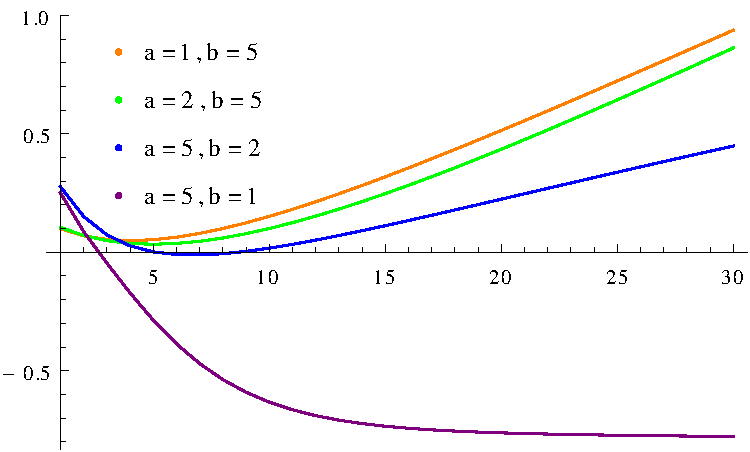
\includegraphics[width = 11cm]{betaGraph.pdf}
\caption{Difference in revenue: $R(r^*, N-1)-R(\hat{r}, N)$} \label{fig:graph}
\end{figure}

\begin{remark}
 Specially for the uniform distribution, we have, when $N\leq 7$, $R(\hat{r}, N)<R(r^*, N-1)$. 
\end{remark}

\subsubsection{Charging Experience fee to extract trade surplus}
 We then consider the case where the seller can charge experience fee. For the seller, at the experience-stage, how to optimally set price of exprience? 
If a certain number of buyers are permitted to experience the good, each of those buyers is supposed to get a nonnegative ex ante expected payoff from participating the
subsequent second-price auction. Suppose that buyers will buy the experience when they are indifferent between remaining
uninformed and buying the experience to be informed. 
 Then the seller should set the price equal to a buyer's ex ante expected payoff of participating the auction to extract all the expected trade surplus. Intuitively, the ex ante expected payoff of experiencing buyers depends on the number of auction partipants. 
%First, we set the prespecified price as $\mu$ for the auction. Then the expected result of the auction can be calculated. \end{comment}



Next, we will offer the formula for the experience fee in the following lemma. 
\begin{lemma}
 The experience fee $P(m)$ can be formulated as 
\begin{equation}
 P(m) = \begin{cases}\int_{\mu}^{\overline{v}}\int_{\mu}^vF^{m-1}(t)\mathrm{d}tf(v) \mathrm{d} v, &\textrm{if}\quad m \leq N-1\\
\int_{\underline{v}}^{\overline{v}}\int_{\underline{v}}^v F^{N-1}(t)\mathrm{d}tf(v) \mathrm{d} v, &\textrm{if}\quad m = N
\end{cases}
\end{equation}


\end{lemma}
\begin{proof}
 When there are $m(\leq n-1)$ buyers knowing one's own value information, the value of the information is
\begin{align*}
P(m)&= \int_{\mu}^{\overline{v}}(\int_{\mu}^v (v-t)\mathrm{d}F^{m-1}(t)+(v-\mu)F^{m-1}(\mu))f(v)\mathrm{d}v \\
&= \int_{\mu}^{\overline{v}}\int_{\mu}^vF^{m-1}(t)\mathrm{d}tf(v)\mathrm{d}v
\end{align*}

$P(N)$ can be formulated as, 
 \begin{align*}
P(N) &= \int_{\underline{v}}^{\overline{v}}\int_{\underline{v}}^v(v-t)\mathrm{d}F^{N-1}(t)\mathrm{d}tf(v)\mathrm{d}v \\
 &= \int_{\underline{v}}^{\overline{v}}\int_{\underline{v}}^v F^{N-1}(t)\mathrm{d}tf(v)\mathrm{d}v
\end{align*}
\end{proof}

\begin{lemma}
As the number of buyers knowing one's own value information increases, the expected value of knowing one's own value information decreases. 
\end{lemma}
Notice that for many distributions and potential buyers' number n, $P(N) < P(N-1)$. In such cases, the seller set price at $P(N)$, and 
the buyers' domininant stratey is to buy the experience. 
Since every buyer knows the true value in the auction and expected gain of every buyer is zero now, the seller can extract full surplus through setting appropriate experience fee. the 
social surplus is maximized and fully extracted by the seller. 



The above reasoning leads to the following conclusion

\begin{thm}

 If the seller can charge fee for letting one buyer know his true value, then the seller will set the price
 $ \int_{\underline{v}}^{\overline{v}}\int_{\underline{v}}^v F^{n-1}(t)\mathrm{d}tf(v)\mathrm{d}v$ to fully extract all the surplus of trade, and the revenue she get is 
 \begin{equation}
 E(V_{(1)}^N)=\int_{\underline{v}}^{\overline{v}} x\mathrm{d}F^N(x) 
 \end{equation}
where $V_{(1)}^N$ denotes the highest bid. 
\end{thm}
 This is the best possible result for the seller, maximizing the trade surplus and minimizing all the buyers' share. 


The example is supposed to shed light on a seller's optimal
sales mechamism design when buyers have identical value distribution about the
experience good, but do not know the private value before the experience. The seller controls the number of buyers to experience. 

When the seller is not able to charge experience fee, her optimal sales mechanism might be to exclude a buyer from experiencing the good, which harms social
 efficiency. When the seller is allowed to charge fee, the result is efficient. However, the defect is that
 all the trade surplus is extracted by the seller. 




 

 

\section{Mechanisms we will discuss}

In this section, I would like to talk about the scope of my
thesis. The main focus will be around mechanisms for dealing with
decentralized information problem. The last chapter is a diversion to
some
mechanisms that are designed for special purpose and under special requirements.4 chapters follow this introductory one.

 Chapter 2 is a review of important results in the literatures of mechanism design and Nash implementation, especially those
impossibility results. These results establish the impossibility of implementability with most general conditions. And this lead us to put effort in the consideration of more specific environments and conditions. The body of theory on Perfect Information Nash implementation exemplify the method mostly employed in the search. They proposed conditions and then through method of construction proved that under the conditions certain social goal can be Nash implemented.

Chapter 3 is a whole chapter devoted to the study of ex post implementation of socially efficient allocation goal through money transfer under the interdependent value environment. The material in this chapter employ the condition-proposing and constructive-proving method frequently found in mechanism design literature. Both continuous and discrete cases are considered. A sufficient condition called Condtion $\rho$ for ex post implementation with interdependent values via money transfer is given for the multiple goods assignment problem as an attempt to contribute to the field. 

Chapter 4 is devoted to a discussion of matching mechanisms design. The attention is later focused on an application of the theory to the Chinese college admission mechanism. A few derived propositions show that the score-dictating mechanism is perhaps the best choice among three popular mechanisms.

Chapter 5 is a chapter reflecting upon a special class of mechanisms in which the implementation goal is to let the side with more skills etc to win. It is up to the agents to show their techniques to compete in these mechanism to win . Focus is put upon finite dynamic games with perfect information with chess as a model for the convenience of discussion.





